\chapter{SSH and Secure Remote Access}

In Chapter~27, we saw how secure messaging protects asynchronous conversations between people across untrusted relays. Remote system administration poses a related problem: protecting a live, interactive session between an engineer and a machine across an untrusted network. SSH, the \emph{Secure Shell}, brings together nearly every primitive we have built so far -- Diffie-Hellman, RSA, elliptic curves, authenticated encryption, hashes, signatures, and certificates -- to answer one practical question: \emph{how do I get a trustworthy command line on a machine that is across the room, across the building, or across an ocean, over a network I do not control?}

When you type \texttt{ssh alice@server.example.com} and a moment later you are looking at a shell prompt on a machine three thousand miles away, an enormous amount of cryptography has just happened in under a second. A fresh key was negotiated over a hostile network. The remote machine proved it is the one you meant to reach. You proved you are allowed in. And every keystroke from that point forward is encrypted and authenticated, immune to a passive eavesdropper and -- if you set it up right -- to an active attacker sitting in the middle. This chapter takes that second apart.

We will meet Alice (you, at your laptop), the server she wants to reach, and Eve, who controls the network in between -- she can read every packet, drop packets, inject packets, and impersonate either endpoint. Our job is to understand exactly what SSH does to defeat her, where the math comes from, and the fragile moment where SSH quietly hands the security decision back to a human and how often that human gets it wrong.

\section{What problem SSH solves}

\begin{historybox}
Before SSH there was \texttt{telnet}, \texttt{rlogin}, \texttt{rsh}, and \texttt{rcp}. All of them sent your password, and then your entire session, in cleartext. On a shared Ethernet segment or a compromised router, anyone running a packet sniffer harvested credentials for free. In 1995 Tatu Ylonen, a researcher at Helsinki University of Technology, watched exactly such a password-sniffing attack run against his network and wrote SSH-1 as a direct replacement. It spread explosively. SSH-1 had real cryptographic flaws (including a CRC-32 integrity check, an unkeyed polynomial checksum that enabled plaintext-insertion attacks), so the protocol was redesigned from scratch as SSH-2, standardized by the IETF in RFCs 4250--4254 (2006). Today ``SSH'' means SSH-2; SSH-1 is dead and should be refused. The dominant implementation, OpenSSH, grew out of the OpenBSD project and now ships on essentially every server on Earth. The primary open challenge today is migrating the installed base to post-quantum hybrid key exchange (combining X25519 with ML-KEM) before store-now-decrypt-later adversaries record traffic for future quantum decryption.
\end{historybox}

The threat model is worth stating precisely, because SSH's whole design follows from it.

\begin{focusbox}
\textbf{Threat model.} The network between Alice and the server is fully controlled by Eve (a \emph{Dolev-Yao} attacker). She can:
\begin{itemize}
  \item read every byte that crosses the wire (passive eavesdropping);
  \item modify, delete, reorder, or replay packets;
  \item insert packets of her own, including pretending to be the server to Alice and pretending to be Alice to the server (an active man-in-the-middle).
\end{itemize}
What Eve \emph{cannot} do: break the underlying primitives (factor RSA moduli, compute discrete logs in the chosen group, find AES keys, find hash collisions in a strong hash), and she cannot read the private keys stored on Alice's laptop or the server. The security goals SSH must meet against this Eve are: \emph{confidentiality} (she learns nothing about the session contents), \emph{integrity} (she cannot alter the session undetected), \emph{server authentication} (Alice reaches the machine she intended, not Eve's impostor), and \emph{client authentication} (only authorized users get a shell).
\end{focusbox}

Notice the asymmetry hiding in ``server authentication.'' For TLS on the web, a certificate authority vouches for \texttt{example.com} so your browser can verify a server it has never seen before. SSH usually has no such authority. That single missing piece -- how Alice knows the server is the real server the very first time she connects -- is the most interesting and most abused part of the whole system, and we will spend a full section on it.

\section{The three layers of SSH}

SSH-2 is deliberately built as three stacked protocols, each with one job. Keeping them separate is what lets you reason about the system at all.

\begin{center}
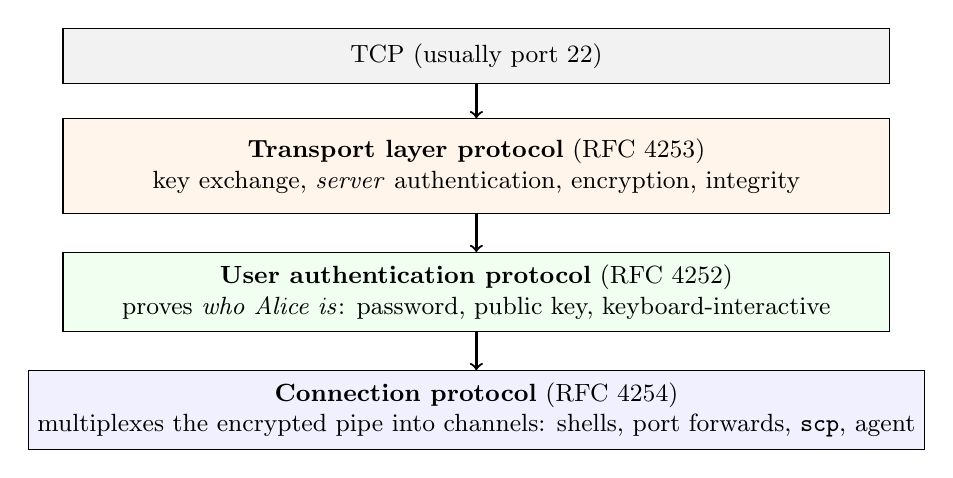
\begin{tikzpicture}[font=\small,every node/.style={align=center}]
  \node[draw, fill=blue!6, minimum width=10.5cm, minimum height=1.0cm] (conn) at (0,0)
    {\textbf{Connection protocol} (RFC 4254)\\ multiplexes the encrypted pipe into channels: shells, port forwards, \texttt{scp}, agent};
  \node[draw, fill=green!6, minimum width=10.5cm, minimum height=1.0cm] (auth) at (0,1.5)
    {\textbf{User authentication protocol} (RFC 4252)\\ proves \emph{who Alice is}: password, public key, keyboard-interactive};
  \node[draw, fill=orange!8, minimum width=10.5cm, minimum height=1.2cm] (trans) at (0,3.1)
    {\textbf{Transport layer protocol} (RFC 4253)\\ key exchange, \emph{server} authentication, encryption, integrity};
  \node[draw, fill=gray!10, minimum width=10.5cm, minimum height=0.7cm] (tcp) at (0,4.5)
    {TCP (usually port 22)};
  \draw[->,thick] (tcp) -- (trans);
  \draw[->,thick] (trans) -- (auth);
  \draw[->,thick] (auth) -- (conn);
\end{tikzpicture}
\end{center}

Read it bottom to top, which is the order events happen:

\begin{enumerate}
  \item \textbf{Transport layer.} Runs first, on the raw TCP connection. It performs the key exchange, authenticates the \emph{server} (via its host key), and from then on encrypts and MAC-protects everything above it. After this layer finishes you have a secure pipe -- but the server still has no idea who you are.
  \item \textbf{User authentication.} Runs \emph{inside} the secure pipe the transport layer built. Now that nobody can eavesdrop, Alice can safely send a password or, far better, prove possession of a private key. This is where \emph{client} authentication lives.
  \item \textbf{Connection protocol.} Once you are authenticated, this layer slices the single encrypted pipe into multiple logical \emph{channels}. One channel carries your interactive shell; another might forward a TCP port; another tunnels your SSH agent. They share the one key-exchanged, encrypted connection.
\end{enumerate}

\begin{intuitionbox}
The layering buys a clean mental model: ``first build a private tunnel and check who's at the far end (transport), then walk through it and show your ID (auth), then do as many things as you like through the tunnel (connection).'' Each layer assumes the one below it already did its job. The most common SSH security failures happen at the boundary between layers one and two -- specifically, Alice accepts the wrong server in layer one and then types her password into Eve's prompt in layer two. An encrypted tunnel without server authentication only gives you a private connection to an impostor.
\end{intuitionbox}

\section{The transport layer: key exchange and host keys}

\subsection{Identification and algorithm negotiation}

The moment the TCP connection opens, both sides send a banner line, in cleartext, like:

\begin{center}\ttfamily SSH-2.0-OpenSSH\_9.6\end{center}

The \texttt{2.0} pins the protocol version (a \texttt{1.x} here would let an old client fall back to broken SSH-1; modern servers simply do not offer it). Then each side sends a \texttt{SSH\_MSG\_KEXINIT} message listing, in preference order, the algorithms it supports for: key exchange, host-key signature, symmetric cipher (each direction), MAC (each direction), and compression. The two ordered lists are reconciled by a deterministic rule -- the chosen algorithm is the client's most-preferred one that the server also supports -- so both ends independently arrive at the same choice without extra round trips.

These \texttt{KEXINIT} messages are sent before any key exists, so they are unencrypted, which means Eve can read them. That is fine; the algorithm names are not secret. But she could \emph{tamper} with them to force a weak choice (a downgrade attack). SSH defends against this by folding the exact bytes of both \texttt{KEXINIT} messages into the key-exchange hash, as we are about to see. If Eve flips a bit, the two sides compute different hashes and the host-key signature fails to verify. The negotiation is unencrypted but not unauthenticated.

\subsection{The key exchange itself}

The classic SSH key exchange is Diffie-Hellman; modern OpenSSH defaults to \emph{Curve25519} (the elliptic-curve DH from Chapter~21) but the structure is identical, so let us write it with plain DH over a prime field $\Z/p\Z$ and a generator $g$, and you can mentally swap in the curve. The server owns a long-term \emph{host key pair} $(\textit{pk}_H, \textit{sk}_H)$ -- this is the key that names the server's identity, and remembering it across connections is the whole trust story of the next section.

\begin{formalbox}
\textbf{SSH Diffie-Hellman key exchange.} Let $V_C, V_S$ be the client and server identification strings, and $I_C, I_S$ the two \texttt{KEXINIT} payloads.
\begin{enumerate}
  \item Client picks $x \getsr \{2,\dots,p-2\}$, computes $e = g^{x} \bmod p$, sends $e$.
  \item Server picks $y \getsr \{2,\dots,p-2\}$, computes $f = g^{y} \bmod p$ and the shared value $K = e^{y} \bmod p$.
  \item Server forms the \emph{exchange hash}
  \[
    H = \Hash\!\left(V_C \concat V_S \concat I_C \concat I_S \concat \textit{pk}_H \concat e \concat f \concat K\right),
  \]
  signs it: $s = \Sign_{\textit{sk}_H}(H)$, and sends $(\textit{pk}_H,\, f,\, s)$.
  \item Client computes $K = f^{x} \bmod p$, reconstructs the \emph{same} $H$ from the values it already has, and verifies $\Vrfy_{\textit{pk}_H}(H, s)$. If the signature checks out, the server is authenticated.
\end{enumerate}
The shared secret is $K$ because $e^{y} = g^{xy} = f^{x} \pmod p$. The session key material is derived from $H$ and $K$ by hashing, described below. The exchange hash $H$ doubles as the \emph{session identifier} for the life of the connection.
\end{formalbox}

\begin{whybox}
Why is this man-in-the-middle proof? Plain Diffie-Hellman is \emph{not} -- Eve can run one DH with the client and another with the server, sitting in the middle and reading everything. The single ingredient that fixes this is the server's signature over $H$. Because $H$ commits to $f$ (the server's DH share) \emph{and} to $\textit{pk}_H$ \emph{and} to both \texttt{KEXINIT} payloads, a valid signature under the host key proves: ``the entity that owns $\textit{sk}_H$ chose this DH share $f$, in the context of these negotiated algorithms.'' If Eve substitutes her own $f' = g^{y'}$ to set up her half of the tunnel, she would have to produce a signature on the corresponding $H'$ under $\textit{sk}_H$ -- which she does not have. Her only escape is to present her \emph{own} host key $\textit{pk}_H'$ and sign with it. The signature will verify mathematically. The protocol cannot stop her here. The defense moves up to the human: \emph{does Alice recognize that host key?} That is trust-on-first-use, and it is the subject of the next section.
\end{whybox}

\begin{connectionbox}
The security of $K$ against a passive Eve is exactly the \emph{computational Diffie-Hellman} assumption from Chapter~18: given $g^{x}$ and $g^{y}$ she cannot compute $g^{xy}$. With Curve25519 the group is the curve's point group of prime order $\approx 2^{252}$, and the best known attack is generic discrete log at cost $\approx 2^{126}$ (Pollard rho, from the algorithms companion). Folding $K$ through a hash to make keys means even the \emph{decisional} DH leakage is laundered into uniform-looking bits. Why hash rather than use $K$ directly? Raw DH outputs are not uniform -- $g^{xy} \bmod p$ lives in a subgroup and has detectable bias -- and a single $K$ must yield several independent keys; hashing fixes both, exactly as the KDF discussion in Chapter~23 argued.
\end{connectionbox}

\subsection{From one secret to six keys}

A session needs more than one key. Each direction (client-to-server and server-to-client) needs an encryption key, a MAC key (when a separate MAC is used), and an initialization vector. SSH derives all of them from the pair $(K, H)$ by repeated hashing, where the letters \texttt{A}--\texttt{F} are literal ASCII tags:

\[
\begin{aligned}
\text{IV}_{C \to S}     &= \Hash(K \concat H \concat \texttt{"A"} \concat \textit{session\_id}) \\
\text{IV}_{S \to C}     &= \Hash(K \concat H \concat \texttt{"B"} \concat \textit{session\_id}) \\
\text{Enckey}_{C \to S} &= \Hash(K \concat H \concat \texttt{"C"} \concat \textit{session\_id}) \\
\text{Enckey}_{S \to C} &= \Hash(K \concat H \concat \texttt{"D"} \concat \textit{session\_id}) \\
\text{MACkey}_{C \to S} &= \Hash(K \concat H \concat \texttt{"E"} \concat \textit{session\_id}) \\
\text{MACkey}_{S \to C} &= \Hash(K \concat H \concat \texttt{"F"} \concat \textit{session\_id})
\end{aligned}
\]

On the very first key exchange, $\textit{session\_id} = H$. If a key is longer than one hash output, SSH extends it by hashing $K \concat H$ concatenated with all key bytes produced so far -- a simple counter-free expansion. The distinct tags \texttt{A}--\texttt{F} guarantee the six outputs are independent even though they all derive from the same $(K,H)$: flipping one tag byte changes the hash input completely. Figure~\ref{ch28:fig-key-derivation} shows how the shared DH secret $K$ and the exchange hash $H$ fan out into the six directional keys and IVs.

\begin{figure}[H]
\centering
\begin{tikzpicture}[font=\scriptsize, >=stealth]
  % Inputs on the left
  \node[draw=aliceblue!80, fill=aliceblue!10, rounded corners=2pt, minimum width=2.8cm, minimum height=0.8cm, align=center] (k) at (0, 1.3) {
    \textbf{Shared Secret $K$}\\
    $g^{xy} \bmod p$
  };
  \node[draw=bobgreen!80, fill=bobgreen!10, rounded corners=2pt, minimum width=2.8cm, minimum height=0.8cm, align=center] (h) at (0, -0.1) {
    \textbf{Exchange Hash $H$}\\
    (also \textit{session\_id})
  };

  % Central KDF box
  \node[draw=structurepurple!80, fill=structurepurple!12, rounded corners=3pt, minimum width=3.4cm, minimum height=2.2cm, align=center] (kdf) at (4.4, 0.6) {
    \textbf{Hash KDF}\\
    $\Hash(K \concat H \concat \text{tag} \concat \textit{session\_id})$\\[3pt]
    Domain separation via\\
    ASCII tags \texttt{"A"}--\texttt{"F"}
  };

  \draw[->, thick, aliceblue!80!black] (k.east) -- (kdf.west |- k.east);
  \draw[->, thick, bobgreen!80!black] (h.east) -- (kdf.west |- h.east);

  % Six outputs on the right
  \node[draw=aliceblue!80, fill=aliceblue!8, rounded corners=2pt, minimum width=3.8cm, minimum height=0.45cm, align=center] (oA) at (9.8, 2.35) {Tag \texttt{"A"} $\to \text{IV}_{C \to S}$};
  \node[draw=bobgreen!80, fill=bobgreen!8, rounded corners=2pt, minimum width=3.8cm, minimum height=0.45cm, align=center] (oB) at (9.8, 1.65) {Tag \texttt{"B"} $\to \text{IV}_{S \to C}$};
  \node[draw=aliceblue!80, fill=aliceblue!14, rounded corners=2pt, minimum width=3.8cm, minimum height=0.45cm, align=center] (oC) at (9.8, 0.95) {Tag \texttt{"C"} $\to \text{Enckey}_{C \to S}$};
  \node[draw=bobgreen!80, fill=bobgreen!14, rounded corners=2pt, minimum width=3.8cm, minimum height=0.45cm, align=center] (oD) at (9.8, 0.25) {Tag \texttt{"D"} $\to \text{Enckey}_{S \to C}$};
  \node[draw=aliceblue!80, fill=aliceblue!8, rounded corners=2pt, minimum width=3.8cm, minimum height=0.45cm, align=center] (oE) at (9.8, -0.45) {Tag \texttt{"E"} $\to \text{MACkey}_{C \to S}$};
  \node[draw=bobgreen!80, fill=bobgreen!8, rounded corners=2pt, minimum width=3.8cm, minimum height=0.45cm, align=center] (oF) at (9.8, -1.15) {Tag \texttt{"F"} $\to \text{MACkey}_{S \to C}$};

  \foreach \dest in {oA, oB, oC, oD, oE, oF} {
    \draw[->, thick, structurepurple!80!black] (kdf.east) -- (\dest.west);
  }
\end{tikzpicture}
\caption{SSH key derivation pipeline. A single Diffie-Hellman shared secret $K$ and exchange hash $H$ are domain-separated by single-byte ASCII tags (\texttt{"A"} through \texttt{"F"}) to produce six independent cryptographic keys and IVs -- three for client-to-server traffic and three for server-to-client traffic.}
\label{ch28:fig-key-derivation}
\end{figure}

\begin{trapbox}
Using \emph{different} keys per direction is not paranoia, it is load-bearing. If the client-to-server and server-to-client streams shared a key and IV, an attacker could reflect a packet back at its sender and, with some cipher modes, learn or forge content. Separate keys per direction also stop trivial replay of a captured packet into the opposite stream. This per-direction, per-purpose key separation is a pattern you will see in TLS, IPsec, and Signal -- never reuse a key for two jobs.
\end{trapbox}

Once both sides have the six keys, the client sends \texttt{SSH\_MSG\_NEWKEYS}, and from the next packet on, every SSH packet is encrypted and integrity-protected. SSH also \emph{rekeys} periodically (after roughly a gigabyte of traffic or an hour, by default) by re-running the key exchange inside the existing encrypted channel, which limits how much data ever rides on a single key and gives a measure of forward secrecy across the rekey boundary.

\subsection{The Binary Packet Protocol: encrypt and MAC}

Every byte above the transport layer is wrapped in a \emph{binary packet}:

\begin{center}
\begin{tikzpicture}[font=\small,node distance=0pt]
  \node[draw,fill=gray!12,minimum height=0.9cm,minimum width=1.8cm] (len) {\shortstack{packet\\length}};
  \node[draw,fill=gray!12,minimum height=0.9cm,minimum width=1.6cm,right=of len] (pad) {\shortstack{pad\\length}};
  \node[draw,fill=blue!8,minimum height=0.9cm,minimum width=3.2cm,right=of pad] (payload) {payload (compressed)};
  \node[draw,fill=orange!10,minimum height=0.9cm,minimum width=2.4cm,right=of payload] (padding) {random padding};
  \node[draw,fill=green!10,minimum height=0.9cm,minimum width=1.8cm,right=of padding] (mac) {MAC};
  \draw[decorate,decoration={brace,amplitude=5pt,mirror},thick]
    (len.south west) -- (padding.south east) node[midway,below=8pt] {encrypted};
  \draw[decorate,decoration={brace,amplitude=5pt},thick]
    (len.north west) -- (padding.north east) node[midway,above=8pt] {MAC over this (plus sequence number)};
\end{tikzpicture}
\end{center}

The padding (4--255 random bytes) rounds the packet up to a cipher-block multiple and hides the exact payload length. The MAC is computed over an implicit 32-bit \emph{packet sequence number} concatenated with the unencrypted packet -- the sequence number is never transmitted, it is just a counter both sides keep, and including it is what makes each packet's MAC unique and prevents replay and reordering. If Eve drops or duplicates a packet, the sequence numbers desynchronize and the next MAC fails.

\begin{attackbox}
\textbf{Encrypt-and-MAC and the 2009 plaintext-recovery attack.} Classic SSH used \emph{Encrypt-and-MAC}: it MACs the plaintext and encrypts separately, and -- worse -- the \emph{packet length field itself was encrypted with CBC mode}, so the receiver had to decrypt the first block just to learn how many more bytes to read. Albrecht, Paterson, and Watson (2009) showed this leaks: by injecting a captured ciphertext block and watching whether the connection produced a length error or a MAC error, and how many bytes it waited for, an attacker could recover 14 to 32 bits of an underlying plaintext block per connection. The fixes that shipped: prefer \emph{CTR} mode (no block-boundary length dependence), prefer dedicated AEAD constructions, and add Encrypt-then-MAC variants (\texttt{*-etm@openssh.com}). Today OpenSSH defaults to \texttt{chacha20-poly1305@openssh.com} (an AEAD that even encrypts the length field with a separate key) or AES-GCM. The lesson generalizes Chapter~16: \emph{Encrypt-and-MAC is the fragile composition; prefer Encrypt-then-MAC or a real AEAD.}
\end{attackbox}

\begin{walkbox}
Trace a tiny exchange. Take the toy group $\Z/23\Z$ with generator $g = 5$. Suppose the client draws $x = 6$ and the server draws $y = 15$.
\begin{itemize}
  \item Client sends $e = 5^{6} \bmod 23$. Compute: $5^2 = 25 \equiv 2$, $5^3 \equiv 10$, $5^6 = (5^3)^2 = 100 \equiv 100 - 4\cdot23 = 8$. So $e = 8$.
  \item Server sends $f = 5^{15} \bmod 23$. Compute: $5^{15} = (5^3)^5 = 10^5 \bmod 23$. $10^2 = 100 \equiv 8$, $10^4 \equiv 8^2 = 64 \equiv 64-46 = 18$, $10^5 \equiv 18 \cdot 10 = 180 \equiv 180 - 7\cdot23 = 19$. So $f = 19$.
  \item Server's secret $K = e^{y} = 8^{15} \bmod 23$. Client's secret $K = f^{x} = 19^{6} \bmod 23$. Check they match: $8^{15} = (g^{x})^{y} = g^{xy} = g^{90}$, and $19^{6} = (g^{y})^{x} = g^{90}$ too. Reduce $g^{90}$: the order of $5$ mod $23$ divides $22$; $5^{22} \equiv 1$, so $g^{90} = g^{90 \bmod 22} = g^{2} = 25 \equiv 2$. Both sides get $K = 2$.
\end{itemize}
Now the server hashes $H = \Hash(\dots \concat \textit{pk}_H \concat 8 \concat 19 \concat 2)$ and signs it. Eve, watching $e=8$ and $f=19$ on the wire, faces the discrete-log problem $5^{x} \equiv 8$, which for these toy numbers she can brute force ($x=6$) but for a 252-bit curve she cannot. The signature over $H$ is what stops her from swapping $f=19$ for her own value.
\end{walkbox}

\section{Host keys and trust on first use}

Here is the part of SSH that is unlike TLS, and the part that bites people.

The server's host key authenticates the server. But where does Alice's laptop learn the \emph{correct} host key? On the web, a certificate authority signs \texttt{example.com}'s key and your browser ships with the CA's key built in, so verification is automatic. Plain SSH has no CA. The first time Alice connects to a new server, her client has nothing to check the host key against. So OpenSSH does the only thing it can: it shows her the key's fingerprint and asks.

\begin{center}\ttfamily
The authenticity of host 'server.example.com (203.0.113.7)' can't be established.\\
ED25519 key fingerprint is SHA256:Zm9vYmFyYmF6cXV4cXV1eGNvcmdlZ3JhdWx0.\\
Are you sure you want to continue connecting (yes/no/[fingerprint])?
\end{center}

If Alice types \texttt{yes}, the client stores the host key in \texttt{\textasciitilde/.ssh/known\_hosts} and \emph{from then on} verifies every future connection against that stored copy. This is \emph{Trust On First Use} (TOFU), also called \emph{key continuity}.

\begin{intuitionbox}
TOFU trades away first-contact security to gain a strong property afterward. The very first connection is vulnerable: if Eve is in the middle right then, she presents her own host key, Alice (who has nothing to compare against) clicks \texttt{yes}, and Eve owns the session. But \emph{every connection after that} is protected, because the real key is now pinned. Eve cannot quietly take over later -- if she swaps the key, Alice's client refuses loudly. TOFU bets that the attacker is not present at the precise instant of first contact, and that the window of one connection is small. For most situations that bet pays off; for high-value targets it does not, which is why the alternatives below exist.
\end{intuitionbox}

\begin{trapbox}
The fingerprint prompt is a real security decision, and clicking \texttt{yes} reflexively defeats the entire point. The fingerprint is a hash of the host key (SHA-256 of the public key in current OpenSSH). To use TOFU correctly, Alice must obtain the genuine fingerprint through an \emph{independent} channel -- a provisioning system, a printed runbook, a phone call to the admin, a value baked into the cloud instance metadata -- and compare it to what the prompt shows. Nobody does this for their personal servers. Almost everybody should do this for production infrastructure.
\end{trapbox}

\begin{attackbox}
\textbf{The host key change warning, and why it is scary.} If a host's key ever differs from the pinned \texttt{known\_hosts} entry, OpenSSH refuses to connect with a wall of warning text:
\begin{center}\ttfamily
WARNING: REMOTE HOST IDENTIFICATION HAS CHANGED!\\
IT IS POSSIBLE THAT SOMEONE IS DOING SOMETHING NASTY!\\
Someone could be eavesdropping on you right now (man-in-the-middle attack)!
\end{center}
This means one of two things. Benign: the server was rebuilt or reinstalled and legitimately has a new key, or its IP was recycled. Malicious: an active man-in-the-middle is presenting a substitute host key right now. The protocol cannot tell these apart -- it just sees a key it did not expect. The dangerous human reaction is to run \texttt{ssh-keygen -R hostname} to delete the old entry and reconnect, accepting the new key. If the cause was actually an attacker, Alice just hand-deleted her only evidence and trusted Eve. The correct response is to verify the new fingerprint out of band \emph{before} deleting anything.
\end{attackbox}

\subsection{Escaping TOFU: certificates and SSHFP}

Two mechanisms remove the first-use gamble.

\textbf{SSH certificates.} OpenSSH supports its own (non-X.509) certificate format. An organization creates one \emph{host CA} key pair, keeps the private part offline, and signs each server's host key, producing a host certificate. Every laptop is configured once with a single line in \texttt{known\_hosts}:

\begin{center}\ttfamily @cert-authority *.example.com ssh-ed25519 AAAA...\end{center}

Now when any server in \texttt{example.com} presents a host certificate signed by that CA, the client verifies the signature and connects -- \emph{no prompt, no TOFU, no per-host pinning}. Clients trust new servers automatically the day they are provisioned. The same machinery signs \emph{user} keys: a user CA issues short-lived certificates (valid for, say, eight hours) tying a public key to a username and an expiry, so the server trusts one CA instead of managing thousands of \texttt{authorized\_keys} files. This is how large fleets (Facebook, Netflix, and others have written about it publicly) run SSH at scale.

\begin{whybox}
SSH certificates convert key continuity into a one-time root of trust, exactly the CA model from Chapter~24 but minus X.509's complexity. The security argument is the signature: a host cert is $\Sign_{\textit{sk}_{CA}}(\textit{pk}_H \concat \textit{principals} \concat \textit{validity})$. A client holding $\textit{pk}_{CA}$ verifies it offline. Eve cannot forge a cert without $\textit{sk}_{CA}$, which lives offline. Short-lived \emph{user} certs are forward-secure in a practical sense: a stolen user key is worthless once the cert expires, so there is no giant \texttt{authorized\_keys} file to audit and no revocation list to distribute for the common case. Revocation, when needed, is a published \texttt{KRL} (key revocation list) the servers load.
\end{whybox}

\textbf{SSHFP DNS records.} You can publish a host key's fingerprint in DNS as an \texttt{SSHFP} record. With DNSSEC signing that record, a client configured with \texttt{VerifyHostKeyDNS=yes} authenticates the host key against signed DNS instead of asking the user. The trust then rests on the DNSSEC chain rather than on a private CA -- useful when you control DNS but do not want to run an SSH CA. Figure~\ref{ch28:fig-tofu-vs-ca} contrasts the vulnerable first-contact window of TOFU against the offline root of trust provided by an SSH host CA.

\begin{figure}[H]
\centering
\begin{tikzpicture}[font=\scriptsize, >=stealth]
  % Left Panel: TOFU
  \draw[draw=quotientorange!80, fill=quotientorange!5, rounded corners=3pt, thick] (0, 0) rectangle (6.6, 3.8);
  \node[font=\footnotesize\bfseries, text=quotientorange!90!black] at (3.3, 3.45) {Trust On First Use (TOFU)};

  \node[draw=aliceblue!80, fill=white, rounded corners=2pt, minimum width=1.8cm, minimum height=0.7cm, align=center] (c1) at (1.2, 2.2) {Client\\(empty list)};
  \node[draw=bobgreen!80, fill=white, rounded corners=2pt, minimum width=1.8cm, minimum height=0.7cm, align=center] (s1) at (5.4, 2.2) {Server\\$\textit{pk}_H$};

  \draw[<-, thick, trapred] (c1.north east) -- node[above, font=\tiny, text=trapred]{1st connect: unverified $\textit{pk}_H$} (s1.north west);
  \draw[->, thick, targetgreen!80!black] (c1.south east) -- node[below, font=\tiny, text=targetgreen!80!black]{2nd+ connect: pinned in \texttt{known\_hosts}} (s1.south west);

  \node[draw=trapred!70, fill=trapred!8, rounded corners=2pt, text width=5.8cm, align=center, font=\tiny] at (3.3, 0.65) {
    \textbf{Risk}: Active MITM on 1st connect can substitute $\textit{pk}_{\text{Eve}}$\\
    if human clicks \texttt{yes} without out-of-band check.
  };

  % Right Panel: SSH CA
  \draw[draw=targetgreen!80, fill=targetgreen!5, rounded corners=3pt, thick] (7.2, 0) rectangle (14.2, 3.8);
  \node[font=\footnotesize\bfseries, text=targetgreen!90!black] at (10.7, 3.45) {SSH Host Certificate (CA Model)};

  \node[draw=structurepurple!80, fill=structurepurple!12, rounded corners=2pt, minimum width=2.2cm, minimum height=0.6cm, align=center] (ca) at (10.7, 2.75) {Offline Host CA\\$(\textit{pk}_{CA}, \textit{sk}_{CA})$};
  \node[draw=aliceblue!80, fill=white, rounded corners=2pt, minimum width=1.6cm, minimum height=0.7cm, align=center] (c2) at (8.2, 1.55) {Client\\pins $\textit{pk}_{CA}$};
  \node[draw=bobgreen!80, fill=white, rounded corners=2pt, minimum width=1.6cm, minimum height=0.7cm, align=center] (s2) at (13.2, 1.55) {Server\\holds Cert};

  \draw[->, dashed, thick, structurepurple] (ca.west) -| node[above, pos=0.25, font=\tiny]{config once} (c2.north);
  \draw[->, dashed, thick, structurepurple] (ca.east) -| node[above, pos=0.25, font=\tiny]{signs $\textit{pk}_H$} (s2.north);
  \draw[<-, thick, targetgreen!80!black] (c2.east) -- node[below=2pt, font=\tiny]{Cert: $\textit{pk}_H + \Sign_{\textit{sk}_{CA}}(\textit{pk}_H)$} (s2.west);

  \node[draw=targetgreen!70, fill=targetgreen!10, rounded corners=2pt, text width=6.2cm, align=center, font=\tiny] at (10.7, 0.55) {
    \textbf{Guarantee}: 1st connect verified automatically against $\textit{pk}_{CA}$;\\
    no human prompt, new hosts trusted immediately.
  };
\end{tikzpicture}
\caption{Comparing Trust On First Use (TOFU) with SSH host certificates. TOFU leaves the very first connection exposed to human error at the fingerprint prompt, whereas an offline Host CA signs each server's host key so clients pinning $\textit{pk}_{CA}$ verify even first contact cryptographically.}
\label{ch28:fig-tofu-vs-ca}
\end{figure}

\section{User authentication: passwords versus public keys}

Once the encrypted, server-authenticated tunnel exists, Alice proves who she is. SSH offers several methods; the two that matter are \emph{password} and \emph{public key}.

\subsection{Password authentication}

The client sends Alice's password to the server through the encrypted tunnel. The server checks it against its user database (hashed with a slow password hash, as Chapter~14 insists). Because the tunnel is encrypted, Eve on the wire learns nothing. So what is wrong with it?

\begin{trapbox}
Password auth has three weaknesses that public keys do not:
\begin{enumerate}
  \item \textbf{The password reaches the server in usable form.} A malicious or compromised server -- or an attacker who fooled Alice past a host-key warning -- receives Alice's actual password and can replay it elsewhere (people reuse passwords). With public keys, the server never sees anything reusable.
  \item \textbf{Online guessing.} The server is exposed to brute-force and credential-stuffing attempts. Internet-facing \texttt{sshd} on port 22 sees thousands of login attempts an hour from botnets. Public keys with no password fallback make guessing pointless: there is nothing to guess in a $2^{256}$ keyspace.
  \item \textbf{Phishing of the secret.} Because the secret is a human-typed string, it can be socially engineered or keylogged. A private key never leaves the laptop.
\end{enumerate}
The standard hardening is \texttt{PasswordAuthentication no} in \texttt{sshd\_config}, allowing only public keys.
\end{trapbox}

\subsection{Public-key authentication}

This is the right way to use SSH. Alice generates a key pair once. The public key goes into \texttt{\textasciitilde/.ssh/authorized\_keys} on every server she may log into; the private key never leaves her laptop (ideally never leaves a hardware token). To log in, she proves she holds the private key by \emph{signing a challenge that is bound to this specific session}.

\begin{formalbox}
\textbf{SSH public-key authentication (publickey method).} Let $(\textit{pk}_U,\textit{sk}_U)$ be Alice's user key pair and $\textit{session\_id} = H$ the transport-layer exchange hash.
\begin{enumerate}
  \item Client sends a \texttt{SSH\_MSG\_USERAUTH\_REQUEST} naming the username, the service, the method \texttt{publickey}, the algorithm, and $\textit{pk}_U$, plus a \emph{signature} $\sigma$.
  \item The signed data is
  \[
    \begin{aligned}
    M = \;&\textit{session\_id} \concat \texttt{USERAUTH\_REQUEST} \concat \textit{username} \concat \textit{service} \\
          &\concat \texttt{"publickey"} \concat \textit{true} \concat \textit{alg} \concat \textit{pk}_U,
    \end{aligned}
  \]
  and $\sigma = \Sign_{\textit{sk}_U}(M)$.
  \item Server checks that $\textit{pk}_U$ appears in this user's \texttt{authorized\_keys}, then verifies $\Vrfy_{\textit{pk}_U}(M,\sigma)$. Both must pass.
\end{enumerate}
\end{formalbox}

\begin{whybox}
Two design points make this secure and they are easy to miss. First, the signature covers $\textit{session\_id} = H$, which is unique to this connection (it contains both fresh DH shares). So $\sigma$ cannot be replayed onto a different connection -- a captured login signature is worthless against tomorrow's session, whose $H$ differs. This is \emph{channel binding}: the auth proof is welded to the exact encrypted tunnel it was made in. Second, the server only ever sees a \emph{signature}, never the private key, so even a fully malicious server learns nothing it can reuse to impersonate Alice elsewhere. Compare password auth, where a malicious server harvests the reusable secret directly. Channel binding plus a non-reusable proof is precisely why public-key auth resists the malicious-server and the man-in-the-middle cases that password auth does not.
\end{whybox}

\begin{connectionbox}
Modern SSH user keys are \texttt{ssh-ed25519} -- the EdDSA signature scheme over Curve25519 from Chapter~22. A key is 32 bytes; a signature is 64 bytes; verification is a couple of curve operations. Ed25519 is deterministic (no per-signature randomness to leak, sidestepping the nonce-reuse catastrophe that broke ECDSA in that chapter) and fast. RSA keys still work but should be at least 3072 bits, and the old \texttt{ssh-dss} (1024-bit DSA) is disabled by default for good reason. Prefer Ed25519; fall back to \texttt{ecdsa} or RSA-3072 only when an old server forces it.
\end{connectionbox}

\begin{implementbox}
A stripped-down sketch of the publickey challenge-response, using Ed25519, to show the \emph{shape} of the protocol -- not a real SSH implementation.

\begin{lstlisting}[language=Python]
# LEARNING ONLY. Not real SSH. No transport encryption here,
# no packet format, no algorithm negotiation. Do not use.
from nacl.signing import SigningKey, VerifyKey
import os

# Alice generates her user key pair once.
sk = SigningKey.generate()
pk = sk.verify_key                      # goes into authorized_keys

# --- transport layer already ran; both sides share session_id H ---
session_id = os.urandom(32)             # stand-in for the exchange hash

def build_signed_blob(session_id, username, pk):
    # Mirrors the M that real SSH signs: bind to THIS session.
    return (session_id
            + b"USERAUTH_REQUEST"
            + username.encode()
            + b"ssh-connection"
            + b"publickey"
            + b"\x01"                    # "true": this is a real signature
            + b"ssh-ed25519"
            + bytes(pk))

# Client side: sign the session-bound blob.
M   = build_signed_blob(session_id, "alice", pk)
sig = sk.sign(M).signature

# Server side: pk must be in authorized_keys AND the signature must verify.
authorized_keys = {bytes(pk)}           # the server's allowlist
def authenticate(username, offered_pk, sig, session_id):
    if bytes(offered_pk) not in authorized_keys:
        return False                    # unknown key: reject
    M = build_signed_blob(session_id, username, offered_pk)
    try:
        VerifyKey(bytes(offered_pk)).verify(M, sig)   # raises on bad sig
        return True
    except Exception:
        return False

print(authenticate("alice", pk, sig, session_id))     # True

# Replay onto a DIFFERENT session fails, because M changes with session_id.
print(authenticate("alice", pk, sig, os.urandom(32))) # False
\end{lstlisting}
The last two lines are the whole point: the same signature authenticates only the session it was made for. Real SSH adds the encrypted transport, the binary packet protocol, and careful canonical encoding of every field. Use OpenSSH, never code like this.
\end{implementbox}

\subsection{Protecting the private key}

A private key sitting in \texttt{\textasciitilde/.ssh/id\_ed25519} is a plaintext credential -- anyone who reads that file becomes Alice. Two layers of defense:

\begin{itemize}
  \item \textbf{Passphrase encryption.} \texttt{ssh-keygen} encrypts the private key file under a passphrase, using a slow KDF (OpenSSH's own \texttt{bcrypt}-based KDF with a configurable round count) so that a stolen file resists offline cracking. A stolen \emph{encrypted} key still needs the passphrase.
  \item \textbf{Hardware-backed keys.} An Ed25519 key can be generated on a FIDO2/U2F security token (\texttt{ssh-keygen -t ed25519-sk}) or stored in a TPM/Secure Enclave. The private key never exists in the laptop's memory; signing happens on the token, often gated by a physical touch. Now even malware with full disk access cannot exfiltrate the key.
\end{itemize}

\section{The agent, and the risk of forwarding it}

Typing a passphrase on every \texttt{ssh}, \texttt{scp}, and \texttt{git push} is intolerable, so the \texttt{ssh-agent} holds decrypted private keys in memory and performs signatures on request. Your terminals talk to the agent over a local Unix socket; you unlock once. The agent never hands out the key -- it only ever returns \emph{signatures}, which is the right design.

\subsection{Agent forwarding}

Now the trap. Alice is logged into server \texttt{A} and from there wants to \texttt{git pull} from a repository or \texttt{ssh} onward to server \texttt{B}, both of which require her key. \emph{Agent forwarding} (\texttt{ssh -A}) makes the agent socket on her laptop reachable from \texttt{A}: processes on \texttt{A} can ask Alice's laptop agent to sign things.

\begin{center}
\begin{tikzpicture}[font=\small,every node/.style={align=center}]
  \node[draw,fill=blue!8,minimum width=2.4cm,minimum height=1cm] (lap) {Alice's\\laptop\\(agent +\\private key)};
  \node[draw,fill=green!8,minimum width=2.4cm,minimum height=1cm,right=3.2cm of lap] (A) {server A\\forwarded\\agent socket};
  \node[draw,fill=orange!8,minimum width=2.4cm,minimum height=1cm,right=3.2cm of A] (B) {server B};
  \draw[<->,thick] (lap) -- node[above]{ssh -A} (A);
  \draw[->,thick] (A) -- node[above,align=center]{onward auth\\via forwarded agent} (B);
  \node[draw,fill=red!12,minimum width=2.2cm,minimum height=0.8cm,below=0.9cm of A] (eve) {root on A\\(or attacker)};
  \draw[->,thick,red!70!black] (eve) -- (A);
\end{tikzpicture}
\end{center}

\begin{attackbox}
\textbf{Forwarded agents are a hijackable signing oracle.} Whoever can read the forwarded agent socket on \texttt{A} -- which includes \texttt{root} on \texttt{A}, and anyone who has compromised \texttt{A} -- can ask \emph{Alice's} agent to sign \emph{anything} for as long as Alice's session is open. They cannot steal the key, but they do not need to: they can use it. While Alice is connected to \texttt{A}, the attacker silently authenticates to \texttt{B}, to \texttt{C}, to her GitHub, to every machine her key opens, all with valid signatures that look exactly like Alice. The moment you \texttt{ssh -A} into a box you do not fully trust, you have lent your identity to its administrator. This has been the pivot point in real breaches.
\end{attackbox}

\begin{whybox}
Use safer mechanisms instead of blanket forwarding:
\begin{itemize}
  \item \textbf{\texttt{ProxyJump} (\texttt{ssh -J bastion target}).} The connection to \texttt{target} is tunneled \emph{through} the bastion, but the bastion only sees ciphertext -- the authentication to \texttt{target} happens end-to-end from your laptop. The bastion never gets access to your agent. This is the correct replacement for ``forward my agent through the jump host.''
  \item \textbf{Confirmation on use (\texttt{ssh-add -c}).} The agent prompts you (a desktop dialog) before every signature, so a hijacker on \texttt{A} cannot sign silently.
  \item \textbf{FIDO2 keys (\texttt{-sk}).} Each signature requires a physical touch, so even a forwarded agent cannot be abused without you tapping the token.
  \item \textbf{Per-host scoping.} If you must forward, scope it to one trusted destination, never \texttt{ForwardAgent yes} globally in \texttt{\textasciitilde/.ssh/config}.
\end{itemize}
\end{whybox}

\section{Port forwarding and the connection layer}

After authentication, the connection protocol multiplexes \emph{channels} over the one encrypted pipe. Beyond the interactive shell, its most heavily used feature is \emph{port forwarding}, which tunnels arbitrary TCP through SSH.

\begin{itemize}
  \item \textbf{Local forward} (\texttt{ssh -L 5432:db.internal:5432 bastion}): your laptop's port 5432 is tunneled, through the SSH connection to \texttt{bastion}, onward to \texttt{db.internal:5432}. You reach an internal database as if it were local, with all traffic encrypted to the bastion.
  \item \textbf{Remote forward} (\texttt{ssh -R 8080:localhost:3000 server}): a port on the \emph{server} forwards back to a service on your laptop -- handy for exposing a local dev server, dangerous if it exposes you.
  \item \textbf{Dynamic forward} (\texttt{ssh -D 1080 server}): SSH acts as a local SOCKS proxy, sending your browser's traffic out through \texttt{server}. A poor man's VPN.
\end{itemize}

Figure~\ref{ch28:fig-port-forwarding} illustrates how local port forwarding encapsulates arbitrary TCP streams
into encrypted SSH channels.

\begin{figure}[H]
\centering
\begin{tikzpicture}[font=\scriptsize, >=stealth]
  % Client Machine
  \draw[draw=aliceblue!80, fill=aliceblue!10, rounded corners=3pt, thick] (-0.5, -0.2) rectangle (2.6, 3.8);
  \node[font=\footnotesize\bfseries, text=aliceblue!90!black] at (1.05, 3.5) {Alice's Laptop};
  
  \node[draw=gray!60, fill=white, rounded corners=1pt, font=\tiny, align=center] (app) at (1.05, 2.7) {Local App / psql\\connects to \texttt{localhost:5432}};
  \node[draw=aliceblue!80, fill=aliceblue!20, rounded corners=2pt, font=\tiny\bfseries, align=center] (ssh_c) at (1.05, 1.2) {SSH Client\\(\texttt{ssh -L 5432:...})};
  \draw[->, thick] (app) -- node[right, font=\tiny]{TCP} (ssh_c);

  % Bastion Server
  \draw[draw=bobgreen!80, fill=bobgreen!10, rounded corners=3pt, thick] (6.1, -0.2) rectangle (9.0, 3.8);
  \node[font=\footnotesize\bfseries, text=bobgreen!90!black] at (7.55, 3.5) {Bastion Server};
  
  \node[draw=bobgreen!80, fill=bobgreen!20, rounded corners=2pt, font=\tiny\bfseries, align=center] (sshd) at (7.55, 1.2) {SSH Daemon\\(\texttt{sshd})};

  % Internal DB Server
  \draw[draw=structurepurple!80, fill=structurepurple!10, rounded corners=3pt, thick] (10.7, 0.2) rectangle (13.6, 3.4);
  \node[font=\footnotesize\bfseries, text=structurepurple!90!black] at (12.15, 3.0) {Private VPC};
  \node[draw=structurepurple!60, fill=white, rounded corners=1pt, font=\tiny, align=center] (db) at (12.15, 1.2) {Internal DB Server\\\texttt{db.internal:5432}};

  % Multiplexed Encrypted SSH Tunnel
  \draw[draw=targetgreen!80, fill=targetgreen!10, rounded corners=2pt, thick] (2.8, 0.2) rectangle (5.9, 2.4);
  \node[font=\tiny\bfseries, text=targetgreen!90!black, align=center] at (4.35, 2.15) {Encrypted Pipe (Port 22)};
  
  % Multiplexed channels inside tunnel
  \draw[->, thick, sourceblue!80] (2.95, 1.55) -- node[above, font=\tiny, text=sourceblue!90!black]{Channel 0: Shell} (5.75, 1.55);
  \draw[->, thick, quotientorange!90!black] (2.95, 1.0) -- node[above, font=\tiny, text=quotientorange!90!black]{Channel 1: Port 5432} (5.75, 1.0);
  \draw[->, thick, gray!80] (2.95, 0.45) -- node[above, font=\tiny, text=gray!80]{Channel 2: SFTP} (5.75, 0.45);

  % Bastion to DB link
  \draw[->, thick, quotientorange!90!black] (sshd) -- node[above=2pt, font=\tiny, fill=white, inner sep=1pt]{Internal TCP} (db);

  % Explanation banner
  \node[draw=gray!50, fill=white, rounded corners=2pt, font=\tiny, align=left, text width=13.5cm] at (6.55, -0.95) {
    \textbf{Local Port Forwarding (\texttt{-L})}: Alice's application connects to a local loopback socket. The SSH client wraps\\
    raw TCP payload into \texttt{SSH\_MSG\_CHANNEL\_DATA} frames inside the encrypted tunnel. The bastion's \texttt{sshd} opens an outbound\\
    TCP connection to the target \texttt{db.internal:5432}, relaying bytes while multiple channels share the single authenticated session.
  };
\end{tikzpicture}
\caption{Port forwarding and channel multiplexing in SSH. A single encrypted and authenticated
TCP connection carries multiple logical channels simultaneously (interactive terminal, file transfer,
and forwarded network ports), securely tunneling traffic to internal services through a bastion host.}
\label{ch28:fig-port-forwarding}
\end{figure}

\begin{applicationbox}
\textbf{Where SSH shows up.} It is the universal remote-administration tool for Linux and Unix servers -- effectively every cloud instance you will ever touch is reached over SSH. \texttt{scp} and \texttt{sftp} ride the same protocol for file transfer. \texttt{git} over SSH (\texttt{git@github.com}) is how most developers push code; the \texttt{git@} login uses your public key and a forced command. Configuration-management tools (Ansible) drive fleets entirely over SSH. Bastion/jump hosts gate access to private networks. The pattern is always the same: one well-analyzed, server-authenticated, public-key-authenticated encrypted channel, reused for shells, files, ports, and version control. When you hear ``connect to the prod box,'' the cryptography underneath is this chapter.
\end{applicationbox}

\section{Common misconfigurations}

The protocol is sound; deployments leak through their settings. The high-value items in \texttt{sshd\_config}:

\begin{attackbox}
\textbf{The misconfiguration checklist.}
\begin{itemize}
  \item \texttt{PermitRootLogin yes} -- lets attackers brute-force the one account that exists on every box and grants full control. Set \texttt{prohibit-password} (key-only root) or \texttt{no}.
  \item \texttt{PasswordAuthentication yes} on an internet-facing host -- exposes every account to online guessing and credential stuffing. Set \texttt{no}; require keys.
  \item Weak or legacy algorithms left enabled -- SSH-1 (never), \texttt{ssh-dss}, \texttt{arcfour}, CBC-mode ciphers, \texttt{hmac-md5}, small DH groups. Pin a modern \texttt{KexAlgorithms}, \texttt{Ciphers}, and \texttt{MACs} list.
  \item World-readable or group-writable \texttt{authorized\_keys}, or a writable \texttt{\textasciitilde/.ssh} -- SSH \emph{silently refuses} keys with loose permissions, and a writable \texttt{authorized\_keys} lets a local attacker add their own key. Lock to \texttt{600}/\texttt{700}.
  \item Stale \texttt{authorized\_keys} entries -- an employee leaves, their key stays, and nobody audits. This is the case SSH certificates with short expiry were invented to kill.
  \item \texttt{ForwardAgent yes} globally -- discussed above; turns every box into an agent-hijack opportunity.
  \item No \texttt{MaxAuthTries}/rate limiting and \texttt{sshd} on the default port wide open -- pair key-only auth with \texttt{fail2ban} or a firewall to cut log noise and slow probing. (Key-only auth is the real defense; rate limiting is hygiene.)
  \item Reused or backed-up \emph{host} keys across many servers -- if one server's host private key leaks, every server sharing it can be impersonated. Each host gets its own key.
\end{itemize}
\end{attackbox}

\begin{intuitionbox}
Step back and the pattern is clear: SSH's cryptography is strong, so attackers go after the seams. The seams are (1) the human at the TOFU prompt, (2) password auth as a guessable fallback, (3) the forwarded agent as a borrowed identity, and (4) stale or over-broad authorization that outlives its purpose. A hardened SSH deployment closes all four: certificate-based host trust (no prompt to fumble), key-only auth (nothing to guess), \texttt{ProxyJump} instead of agent forwarding (no borrowed identity), and short-lived certificates (authorization that expires on its own). Notice none of those fixes touch the math -- they fix where the math hands control back to people.
\end{intuitionbox}

\section{Putting it together}

A full \texttt{ssh alice@server} from cold start runs the message flow in Figure~\ref{ch28:fig-handshake}, in order:

\begin{figure}[H]
\centering
\begin{tikzpicture}[font=\scriptsize, >=stealth]
  % Party boxes
  \node[draw=aliceblue!80, fill=aliceblue!15, rounded corners=2pt, minimum width=2.6cm, minimum height=0.7cm, align=center] (cl) at (0, 0) {
    \textbf{Client (Alice)}\\
    {\tiny Checks \texttt{known\_hosts}}
  };
  \node[draw=bobgreen!80, fill=bobgreen!15, rounded corners=2pt, minimum width=2.6cm, minimum height=0.7cm, align=center] (sv) at (9.0, 0) {
    \textbf{Server (Bob)}\\
    {\tiny Holds Host Key $(pk_H, sk_H)$}
  };

  % Phase 1: Banner & Negotiation
  \draw[->, thick, aliceblue!80!black] (0, -0.7) -- node[above, font=\tiny]{1. Banner: \texttt{SSH-2.0-OpenSSH\_9.6}} (9.0, -0.7);
  \draw[<-, thick, bobgreen!80!black] (0, -1.2) -- node[above, font=\tiny]{2. Banner: \texttt{SSH-2.0-OpenSSH\_9.6}} (9.0, -1.2);

  \draw[->, thick, aliceblue!80!black] (0, -1.8) -- node[above, font=\tiny]{3. \texttt{SSH\_MSG\_KEXINIT} (ciphers, KEX algorithms, MACs)} (9.0, -1.8);
  \draw[<-, thick, bobgreen!80!black] (0, -2.3) -- node[above, font=\tiny]{4. \texttt{SSH\_MSG\_KEXINIT} (ciphers, KEX algorithms, MACs)} (9.0, -2.3);

  % Phase 2: Diffie-Hellman Key Exchange
  \draw[->, thick, aliceblue!80!black] (0, -3.0) -- node[above, font=\tiny]{5. \texttt{SSH\_MSG\_KEXDH\_INIT}: $e = g^x \bmod p$} (9.0, -3.0);
  
  \node[draw=bobgreen!70, fill=bobgreen!10, rounded corners=2pt, font=\tiny, align=center] (sbox1) at (9.0, -3.85) {
    Compute $K = e^y \bmod p$\\
    $H = \Hash(V_C \concat V_S \concat I_C \concat I_S \concat pk_H \concat e \concat f \concat K)$\\
    Sign: $s = \Sign_{sk_H}(H)$
  };

  \draw[<-, thick, bobgreen!80!black] (0, -4.8) -- node[above, font=\tiny]{6. \texttt{SSH\_MSG\_KEXDH\_REPLY}: $pk_H$, $f = g^y \bmod p$, Signature $s$} (9.0, -4.8);

  \node[draw=aliceblue!70, fill=aliceblue!10, rounded corners=2pt, font=\tiny, align=center] (cbox1) at (0, -5.65) {
    Compute $K = f^x \bmod p$, recompute $H$\\
    Verify $\Vrfy_{pk_H}(H, s)$ \& check \texttt{known\_hosts}\\
    Derive 6 directional keys from $(K, H)$
  };

  % Phase 3: NEWKEYS
  \draw[->, thick, aliceblue!80!black] (0, -6.6) -- node[above, font=\tiny]{7. \texttt{SSH\_MSG\_NEWKEYS}} (9.0, -6.6);
  \draw[<-, thick, bobgreen!80!black] (0, -7.05) -- node[above, font=\tiny]{8. \texttt{SSH\_MSG\_NEWKEYS}} (9.0, -7.05);

  % Security Boundary Banner
  \node[draw=structurepurple!80, fill=structurepurple!10, rounded corners=2pt, font=\tiny\bfseries, text=structurepurple!90!black, align=center, minimum width=11.6cm] (banner) at (4.5, -7.6) {
    $\equiv$ Authenticated \& Encrypted Channel Established (Session ID $= H$) $\equiv$
  };

  % Phase 4: User Authentication & Channel Open
  \draw[->, thick, structurepurple] (0, -8.25) -- node[above, font=\tiny]{\texttt{SSH\_MSG\_USERAUTH\_REQUEST} (publickey, $pk_{\text{user}}$, $\Sign_{sk_{\text{user}}}(H \concat \dots)$)} (9.0, -8.25);
  \node[draw=bobgreen!70, fill=bobgreen!10, rounded corners=2pt, font=\tiny, align=center] (sbox2) at (9.0, -8.75) {Check \texttt{authorized\_keys} \& verify signature};
  \draw[<-, thick, structurepurple] (0, -9.3) -- node[above, font=\tiny]{\texttt{SSH\_MSG\_USERAUTH\_SUCCESS}} (9.0, -9.3);

  \draw[->, thick, structurepurple] (0, -9.8) -- node[above, font=\tiny]{\texttt{SSH\_MSG\_CHANNEL\_OPEN} (session $\to$ shell / pty)} (9.0, -9.8);

  % Lifelines drawn between boxes so they never cross text
  \draw[thick, gray!50] (cl.south) -- (cbox1.north);
  \draw[thick, gray!50] (cbox1.south) -- (0, -7.35);
  \draw[thick, gray!50] (0, -7.85) -- (0, -10.0);

  \draw[thick, gray!50] (sv.south) -- (sbox1.north);
  \draw[thick, gray!50] (sbox1.south) -- (9.0, -7.35);
  \draw[thick, gray!50] (9.0, -7.85) -- (sbox2.north);
  \draw[thick, gray!50] (sbox2.south) -- (9.0, -10.0);
\end{tikzpicture}
\caption{The full SSH-2 protocol sequence. Unauthenticated banners and algorithm lists are folded
into the exchange hash $H$ and signed by the server's host key. Once keys are activated via
\texttt{NEWKEYS}, user public-key authentication and multiplexed channels operate inside the secure tunnel.}
\label{ch28:fig-handshake}
\end{figure}

In words:

\begin{enumerate}
  \item TCP connects to port 22; both sides exchange \texttt{SSH-2.0} banners.
  \item \texttt{KEXINIT} negotiates key exchange, host-key signature, cipher, MAC, compression -- client preference wins among mutual support.
  \item Diffie-Hellman (Curve25519) runs; the server signs the exchange hash $H$ with its host key. The client verifies the signature and checks $\textit{pk}_H$ against \texttt{known\_hosts} (TOFU or certificate). \emph{Server authenticated.}
  \item Both sides derive six keys from $(K,H)$, send \texttt{NEWKEYS}; the channel is now encrypted and integrity-protected.
  \item User authentication runs inside the tunnel: Alice signs a session-bound blob with her private key; the server checks \texttt{authorized\_keys} and the signature. \emph{Client authenticated.}
  \item The connection protocol opens a session channel; the server allocates a pseudo-terminal and spawns Alice's shell.
  \item Every keystroke and every byte of output rides the binary packet protocol -- AEAD-encrypted, sequence-numbered, MAC-checked. After about a gigabyte or an hour, the key exchange reruns to rekey.
\end{enumerate}

That is the whole machine: Diffie-Hellman for the secret, a host-key signature to authenticate the server, key continuity (or a certificate) to decide whether to trust that host key, a session-bound user signature for the client, and an AEAD binary packet protocol carrying the rest. Every piece is something you have already met in earlier chapters; SSH is where they snap together into the tool you will actually live in as a working engineer.

SSH secures point-to-point connections over IP networks where endpoints are computers with rich operating systems and filesystems. In the next chapter, we look at cellular networks, where tiny tamper-resistant SIM cards, radio towers, and resource-constrained handsets must authenticate and encrypt traffic at line rate from 2G to 5G.

\section{Exercises}

\begin{exercise}
In the toy group $\Z/23\Z$ with $g = 5$, the client picks $x = 9$ and the server picks $y = 4$. Compute the client's public value $e = g^x$, the server's $f = g^y$, and the shared secret $K$ two ways ($e^y$ and $f^x$) to confirm they agree. Use $5^{22}\equiv 1$ to reduce exponents mod $22$.
\end{exercise}

\begin{exercise}
Explain precisely why a passive Eve who records $e$ and $f$ in the previous exercise cannot recover $K$ when the group is a 252-bit elliptic curve, but can when the group is $\Z/23\Z$. Name the underlying hardness assumption and the best known attack cost.
\end{exercise}

\begin{exercise}
The six SSH session keys are derived as $\Hash(K \concat H \concat t \concat \textit{session\_id})$ for tag bytes $t \in \set{\texttt{A},\dots,\texttt{F}}$. Argue why an attacker who somehow learns $\text{Enckey}_{C\to S}$ (tag \texttt{C}) still learns nothing about $\text{MACkey}_{C\to S}$ (tag \texttt{E}). Which property of $\Hash$ are you relying on?
\end{exercise}

\begin{exercise}
A junior admin reflexively runs \texttt{ssh-keygen -R server} and reconnects whenever the ``REMOTE HOST IDENTIFICATION HAS CHANGED'' warning appears. Describe a concrete attack this habit enables, and the out-of-band step that would have caught it. Why can the SSH protocol itself not distinguish the benign from the malicious cause?
\end{exercise}

\begin{exercise}
Show that the SSH \texttt{publickey} signature cannot be replayed from one connection onto another. Identify exactly which field in the signed blob $M$ guarantees this, and trace what would have to be equal between two connections for a replay to succeed.
\end{exercise}

\begin{exercise}
Alice runs \texttt{ssh -A} into a shared bastion she does not administer, then opens a long-lived session and walks away. The bastion's root user is malicious. Describe step by step what root can do during that session, what root \emph{cannot} do, and how \texttt{ProxyJump} or \texttt{ssh-add -c} would each have prevented or limited the damage.
\end{exercise}

\begin{exercise}
Classic SSH used Encrypt-and-MAC with the CBC-mode packet-length field encrypted. Sketch why the receiver's behavior (waiting for $N$ more bytes versus emitting a MAC error) leaks plaintext bits when an attacker injects a captured ciphertext block. State the two countermeasures OpenSSH adopted and why each removes the leak.
\end{exercise}

\begin{exercise}
Your organization has 4{,}000 servers and 300 engineers. Compare two trust models: (a) every engineer's public key in every server's \texttt{authorized\_keys}, with TOFU host keys; (b) one host CA and one user CA issuing eight-hour user certificates. For each model, state how a new server is trusted by laptops, how a departing engineer is deprovisioned, and the worst-case blast radius of a single leaked private key. Which model scales, and why?
\end{exercise}

\begin{exercise}
Give three distinct reasons public-key authentication resists a malicious or compromised server that password authentication does not. For each, point to the specific mechanism (what the server does or does not receive) that makes the difference.
\end{exercise}

\begin{exercise}
The transport-layer exchange hash is $H = \Hash(V_C \concat V_S \concat I_C \concat I_S \concat \textit{pk}_H \concat e \concat f \concat K)$, signed by the host key. Suppose Eve tampers with the client's \texttt{KEXINIT} ($I_C$) on the wire to force a weaker cipher. Trace, step by step, where the two sides' computations diverge and at which exact check the attack is detected.
\end{exercise}
